\documentclass[10pt,a4paper]{article}
\usepackage[utf8]{inputenc} % para poder usar tildes en archivos UTF-8
\usepackage[spanish]{babel} % para que comandos como \today den el resultado en castellano
\usepackage{a4wide} % márgenes un poco más anchos que lo usual
\usepackage[conEntregas]{caratula}
\usepackage{amsmath} % plain text
\usepackage{verbatim}%
\usepackage{graphicx} % figuras
\usepackage{subfigure} % subfiguras

\begin{document}

\titulo{Tierra Pirata}
\subtitulo{Trabajo Práctico III - Programación de sistemas}

\fecha{\today}

\materia{Organización del Computador II}
\grupo{Grupo: Ariane 5}

\integrante{Greco, Luis}{150/15}{luifergreco@gmail.com}
\integrante{Hertzulis, Nicolás}{811/15}{nicohertzulis@gmail.com}
\integrante{Ramos, Ricardo}{841/11}{riki\_german@yahoo.com.ar}
% Pongan cuantos integrantes quieran

\maketitle

\tableofcontents

\newpage

\section{Introducción}
Un sistema operativo es el conjunto de programas de un dispositivo informático (laptop, celular, etc.) que maneja los recursos de hardware y provee servicios a los programadores de aplicaciones mediante interrupciones de software. Los sistemas operativos se ejecutan en modo privilegiado, aunque puede que una parte se ejecute en modo usuario.\newline
El núcleo o kernel es la parte más fundamental del sistema operativo, que se encarga de hacer los primeros pasos para el arranque del sistema y de proveer las rutinas de atención a interrupciones de software, que utilizan los programadores de aplicaciones.\newline
El kernel se define como la parte del sistema operativo que se ejecuta en modo privilegiado.​\newline
En este trabajo educativo nos proponemos hacer un sistema operativo muy básico para entender los fundamentos de la programación de sistemas operativos.\newline
Para ello completamos diversos fragmentos de un esqueleto de kernel provisto por los docentes. 


\section{Desarrollo}
\subsection{Ejercicio 1}

\subsubsection{Segmentos de código, datos y de pantalla}
El sistema operativo utiliza dos segmentos de código de nivel 0 y 3, dos segmentos de datos de nivel 0 y 3 y un segmento que describe el área de la pantalla de video. Declaramos los cinco segmentos en la Tabla de Descriptores Globales (GDT), cada uno con su correspondiente descriptor. La GDT es un arreglo en memoria cuyas entradas ocupan 64 bits y tienen una estructura particular (ver figura 1). Para ingresar los datos con comodidad utilizamos un struct de C. La primer entrada está ubicada en la posición con índice 8. Todos los segmentos excepto el de video direccionan los primeros 500 MB de la memoria, es decir que se superponen.\newline
\begin{figure}[h]
\centering
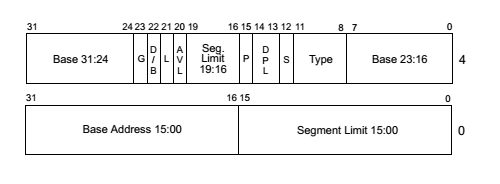
\includegraphics[scale=0.6] {descriptor_segmento}
\caption{Descriptor de segmento.}
\end{figure}
\begin{itemize}
\item Base, límite y granularidad: La base es 0x0, el límite es 0x1F3FF y la granularidad es 1. La granularidad activada hace que tratemos a la memoria como bloques de 4K, por lo tanto el límite con granularidad corresponde a la cantidad de bloques de 4K menos uno. Para direccionar los primeros MB, necesitamos la base en cero. El límite es 0x1F3FF porque en decimal es 127999, ya que necesitamos 128000 bloques de 4KB para llegar a 500 MB. Todo esto es para los segmentos de código y datos. Para descriptor de segmento de pantalla debemos especificar como base \verb|0xB8000| y para el límite necesitamos resolver (80 * 50 * 2) - 1, donde 80 es la cantidad de celdas, 1 celda == 2 bytes, en fila de pantalla y 50 es cantidad de celdas en columna. Es decir que el límite nos la cantidad de bytes que necesitamos para escribir en cualquier parte de la pantalla. Luego el valor del límite es \verb|0x1F3F|. La granularidad está cero ya que tiene menor tamaño (no necesita bloques de 4KB para direccionar toda su memoria).
\item Tipo: 0x0A en los segmentos de código (lectura, ejecución) y 0x02 en los segmentos de datos y de video (lectura, escritura).
\item Nivel de privilegios: 0x0 en los segmentos de datos y código que utiliza en kernel, así como en el segmento de video (que también es de uso exclusivo del kernel). Estos son los segmentos de nivel cero mencionados anteriormente. 0x03 en los segmentos de código y datos que utilizan las tareas, o sea el usuario, que corresponden a los segmentos de nivel tres mencionados anteriorente.
\item Sistema: 0x1 (que significa desactivado) pues no son segmentos de sistema sino de código y datos.
\item Presente: 0x1.
\end{itemize}

\subsubsection{Modo protegido y pila del kernel}
Realizamos los siguientes pasos:
\begin{itemize}
\item Habilitar A20 para poder acceder a direccioner superiores a $2^{20}$ bits.
\item Inicializar la GDT, cuyas entradas fueron ingresadas a partir de una dirección de memoria arbitraria, mediante la instrucción lgdt.
\item Activar el bit menos significativo de CR0.
\item Saltar a segmento:modoprotegido, donde segmento corresponde al índice del segmento de código de nivel 0 en la GDT corrido 3 ceros a la izquierda y modoprotegido corresponde a la dirección de memoria donde arranca el código que se ejecutará a continuación (ya en modo protegido).
\item Establecer los registros selectores de segmento datos (ds, es, gs y ss) en el índice del segmento de datos de nivel cero en la GDT corrido 3 bits a la izquierda.
\item Establecer el registro selector de segmento de video (fs) en el índice del segmento de video en la GDT corrido 3 bits a la izquierda.
\item Establecer la base de la pila en 0x27000.
\end{itemize}

\subsubsection{Limpieza e inicialización de la pantalla}
Para limpiar la pantalla hicimos una función en ensamblador que utiliza el segmento de video y otra en C que utiliza el segmento de datos. La función en ensamblador recorre byte por byte y la función en C recorre celda por celda (2 bytes) y llama a la función screen\_pintar en cada iteración. Ambas funciones dejan la pantalla en negro.\newline
Para inicializar la pantalla llamamos a la función screen\_inicializar que fue completada por nosotros, llamando a la función para limpiar la pantalla y luego a la función screen\_pintar\_rect para las distintas secciones.


\subsection{Ejercicio 2}
\subsubsection{Rutinas de atención a las excepciones del procesador}
Cada interrupción debe tener su entrada en la Tabla de Descriptores de Interrupción (IDT). Las primeras 32 posiciones de esta tabla (índices 0 a 31) corresponden a las excepciones del procesador.\newline
Así como en la GDT, para las entradas de la IDT utilizamos un struct de C, cuyos campos y valores son los siguientes:
\begin{itemize}
\item Selector de segmento: 0x40 que corresponde al índice del segmento de código del kernel en la GDT corrido 3 bits a la izquierda (índice 8).
\item Desplazamiento: La dirección donde comienza el código de la rutina de atención. Es una dirección distinta para cada rutina. Las rutinas están definidas con una macro en ensamblador cuyas etiquetas están declaradas como símbolos globales para poder referenciarlas luego desde C.
\item Atributo: Es un campo que agrupa varios valores. En nuestro caso el valor es 0x8E00. El 8 es un valor hexadecimal que en binario es 1000. El 1 es el bit de presente, los dos bits siguientes son el DPL (nivel 00) y el bit menos significativo debe estar en cero para interrupciones. La E también es un valor hexadecimal que corresponde al $gate type$ y en este caso significa puerta de interrupción de 32 bits.  Así, el valor de atributo es 0x8E y luego se agregan dos ceros a la derecha porque debe estar corrido siempre 8 bits (los ceros son fijos).
\end{itemize}
Las entradas de la IDT se cargan desde una dirección de memoria arbitraria. Una vez cargadas, inicializamos la IDT utilizando la instrucción lidt (load IDT).\newline
Las rutinas solo muestran el número de excepción (que corresponde al índice de la IDT) y luego quedan en un ciclo infinito.

\subsection{Ejercicio 3}
\subsubsection{Paginación}
La paginación es un mecanismo que permite tratar a la memoria en bloques de tamaño fijo, que en este caso son de 4KB y asignar las direcciones físicas de cada página a un rango de mismo tamaño de memoria virtual.\newline Un rango de direcciones de tamaño de una página de memoria virtual puede estar asignado a distintas páginas de memoria física, cada asignación en un directorio de páginas distinto.
\newline Un directorio de páginas tiene 1024 entradas que corresponden a 1024 tablas de páginas. Una tabla de páginas tiene 1024 entradas que corresponden a 1024 páginas.

\subsubsection{Directorio y tablas de páginas del kernel}
El kernel tiene su propio directorio de páginas ubicado en la dirección física 0x27000. Este se va a encargar de las páginas de la zona del kernel, que corresponde a las direcciones físicas 0x00000000 a 0x003FFFFF. Estas direcciones serán asignadas a otras direcciones de memoria virtual, que casualmente en este caso coinciden con las direcciones físicas, por eso decimos que es la asignación identidad, pues la función de asignación es la función identidad.\newline
Para asignar la memoria debemos calcular cuántas páginas necesitamos. Para eso hacemos la siguiente cuenta: (0x003FFFFF + 0x1) / 0x1000 que es igual a 0x400. 0x1000 es el tamaño de una página (en decimal es 4096 pues una página es de 4KB). El resultado 0x400 en decimal es 1024. Por lo cual necesitamos 1024 páginas para completar la zona del kernel. Casualmente 1024 es el tamaño de una tabla de páginas, por lo cual el directorio de páginas del kernel tendrá todas las entradas vacías excepto la primera, que hará referencia a una tabla que estará completamente llena. La tabla de páginas estará en la dirección física 0x28000.\newline
La función que se encarga de inicializar el directorio del kernel es la función $mmu\_inicializar\_dir\_kernel$ y realiza los siguientes pasos:
\begin{itemize}
\item Llenar las 1024 entradas del directorio en cero. En particular el bit de presente está en cero, que en nuestro sistema operativo significa que la memoria correspondiente a esa tabla no está asignada.
\item Modificar la primera entrada con los siguientes valores: 1) Bit de presente activado. 2) Bit de lectura-escritura activado. 3) Base en 0x27 que es la dirección física de la tabla (0x27000) corrida 12 bits a la derecha.
\item Para cada entrada de la tabla, poner una entrada con los siguientes valores: 1) Bit de presente activado. 2) Bit de lectura-escritura activado. 3) Base en el valor i donde i es un número entero entre 0 y 1023. La dirección física es en realidad (i $<<$ 12), pero como luego hay que volverla a correr 12 bits para ingresarla a la estructura, (i $<<$ 12) $>>$ 12 es equivalente a i.
\end{itemize}

\subsubsection{Activación de paginación}
Para tener el mecanismo de paginación funcionando, realizamos los siguientes pasos:
\begin{itemize}
\item Realizar las asignaciones de memoria deseadas (como mínimo la zona del kernel) tal como explicamos en la sección anterior. En nuestro sistema operativo lo hacemos llamando a $mmu\_inicializar\_dir\_kernel$.
\item Poner la dirección física del directorio en el registro de control 3 (CR3).
\item Activar el bit más significativo del registro de control 0 (CR0). Este es el paso que activa el mecanismo.
\end{itemize}
Durante la ejecución del sistema operativo se pueden modificar las asignaciones de memoria del directorio en uso o de otros directorios.


\subsection{Ejercicio 4}

\subsubsection{Manejador de memoria}
Tenemos un manejador de memoria al que le podemos pedir una página libre. El mecanismo es muy básico. Tenemos una variable inicializada en la posición física 0x100000. Cuando alguien llama a la función para pedir la dirección de una página libre, el manejador devuelve el valor de esta variable y luego la incrementa en 0x1000 que es el tamaño de una página, así en la próxima llamada a la función se devuelve la página que está inmediatamente más abajo, que se asume libre.\newline
Con este mecanismo, si borramos una página física de todos los directorios la misma no podrá volver a ser asignada nuevamente, porque el manejador no se enterará que está libre, ya que la variable de la próxima página libre siempre crece.

\subsubsection{Asignación de páginas}
La función mmu\_mapear\_pagina se encarga de asignar un rango de direcciones de memoria virtual a memoria física en un directorio determinado, siendo ese rango el correspondiente a una página. Las direcciones físicas asignadas serán, por lo tanto, el rango [A, A+0x999] donde A es la dirección de comienzo de la página (múltiplo de 0x1000) y 0x999 es 0x1000 - 0x1. No se puede asignar un bloque de memoria menor a una página. Si una página no es suficiente, se puede llamar a esta función tantas veces como sea necesario con distinta páginas. Notar que no es necesario que las páginas físicas sean continuas, pues solo importa que las direcciones virtuales sean contiguas.\newline 
Esta función, entonces, recibe los siguientes parámetros:
\begin{itemize}
\item Dirección física de comienzo de la página (múltiplo de 0x1000).
\item Dirección virtual con la que se desea hacer la asignación.
\item Dirección virtual del directorio de páginas en donde se desea hacer la asignación.
\end{itemize}
Pasos que realiza la función para hacer la asignación:
\begin{itemize}
\item Tomar los 10 bits más significativos de la dirección virtual que corresponden al número de tabla en el directorio de tablas.
\item Tomar los 10 bits siguientes de la dirección virtual que correspondenal número de página en la tabla de páginas.
\item Los 12 bits menos significativos corresponen al desplazamiento dentro de la página, que se usan en el mecanismo de paginación para poder acceder a direcciones particulares dentro de una página. En este caso los desestimamos porque siempre se asigna la página en bloque (solo necesitamos la dirección de comienzo).
\item Si la entrada en el directorio de páginas correspondiente a la tabla (accedemos con el número de tabla calculado anteriormente) tiene el bit de presente activado, obtenemos la dirección de la tabla de páginas.
\item Si no está presente, establecemos como dirección de tabla una dirección de página libre que le pedimos al manejador de memoria y activamos el bit de presente. Las 1024 entradas de esta nueva tabla las inicializamos vacías (en cero).
\item Ahora que tenemos la dirección de la tabla, accedemos a la entrada correspondiente a la página utilizando el número de página calculado al comienzo y pisamos los siguientes valores: activamos bit de presente y ponemos como dirección base la dirección física de la página que recibimos como parámetro.
\item Finalmente llamamos a una función para invalidar la cache de traducción de direcciones.
\end{itemize}

\subsubsection{Eliminación de páginas}
La función mmu\_desmapear\_pagina se encarga de hacer que una página deje de pertenecer a un directorio determinado. Para hacer esto, simplemente separamos la dirección virtual en número de tabla y número de página como en la asignación, accedemos a la tabla desde el directorio y desactivamos el bit de presente de la página correspondiente desde la tabla. Adicionalmente, si detectamos que la tabla queda vacía (todas las entradas con el bit de presente desactivado), desactivamos el bit de presente de la tabla desde el directorio. Por último, llamamos a una función para invalidar la cache de traducción de direcciones.

\subsubsection{Directorios de las tareas pirata}
La función mmu\_inicializar\_dir\_pirata se encarga de crear el directorio para una tarea pirata.\newline
Recibe como parámetros:
\begin{itemize}
\item Dirección física de la página donde se encuentra el código la tarea (se asume que entra en una sola página).
\item Dirección física de destino del pirata (debería ser parte del mapa).
\item ID del pirata.
\end{itemize}
Realiza los siguientes pasos:
\begin{itemize}
\item Pedir al manejador de memoria la dirección de una página libre que utilizaremos para el directorio.
\item Asignar las páginas correspondientes a la zona del kernel en el nuevo directorio. Esto es para poder atender interrupciones.
\item Asignar las páginas en posiciones matricialmente contiguas a la dirección de destino del código en el directorio actual pero usando una tabla de páginas compartida, lo cual hace que estas páginas sean visibles para todas las tareas automáticamente.
\item Copiar el código del pirata de la dirección física de origen a la dirección física destino. Para hacer el copiado del código es necesario asignar una dirección virtual libre cualquiera que esté en la zona de kernel a la dirección física de destino del pirata y usar esta dirección temporal para copiar. Esto es necesario porque para hacer el copiado no usamos el nuevo directorio, sino el directorio actual, que puede pertenecer a otro pirata y si hacemos el copiado usando directamente la dirección virtual 0x400000 estaríamos perdiendo la asignación de ese posible pirata.
\item Luego de hacer el copiado, eliminar esta página temporal del directorio actual y asignar la dirección 0x400000 en el nuevo directorio.
\item Devolver la dirección física del directorio de páginas de la tarea.
\end{itemize}

\subsection{Ejercicio 5}

\subsubsection{IDT}
Inicializamos tres nuevas entradas en la $idt$: la 32, 33 y 70. Las dos primeras con campo $dpl$ en $0x0$, indicando que pueden ser accedidas por el kernel solamente, y la última con $dpl$ en $0x3$, para que pueda
ser accedida por los usuarios.\\
Debemos remapear las direcciones de las interrupciones 32 y 33 porque caen en índices de excepciones del
procesador. Para esto llamamos a función $resetear$ $pic$. Luego habilitamos las interrupciones externas 
llamando a la función $habilitar$ $pic$ que setea flag en registro de control.\\
Para las rutinas de atención 32, 33 y 70 debemos resguardar los registros de uso general de manera que 
las interrupciones sean transparentes a la tarea interrumpida. Luego, excepto en la rutina 70, se debe comunicar al $PIC$ que la interrupción
 será atendida. Esto se hace llamando a la función $fin$ $intr$ $pic1$. Al salir de la rutina se debe restaurar
los registros y ejecutar la instrucción $iret$.\\
La interrupción del reloj solo debe invocar una función, en este caso $game$ $tick$. En cambio la rutina 
del teclado debe leer del puerto $0x60$ la información de la tecla. Esto se hace con la instrucción $in$ en un
registro, por ejemplo $in$ $ax$ , $0x60$.


\subsection{Ejercicio 6}

\subsubsection{TSS}
Para intercambiar tareas necesitamos una tarea inicial, en realidad sólo su estructura de $tss$, para que al switchear se guarde el contexto actual y se pueda cargar el nuevo contexto, registros generales, selectores
 de segmento, registros de control y flags. Entonces inicializamos la $tss$ inicial generando un descriptor 
de $tss$ de la siguiente forma:
\begin{itemize}
\item campo $limite$ en $0x67$ (mínimamente).
\item campo $base$ (separado en una $word$ y dos $bytes$) con dirección de estructura de $tss$ inicial.
\item campo $tipo$ en $0x9$.
\item campo $bit$ system en $0x0$ (es descriptor de sistema).
\item campo $dpl$ en $0x0$ (nivel 0 para que tareas de nivel 3 no puedan saltar a esta).
\item campo $presente$ en $0x1$ (descriptor presente).
\item campos $avl$, $db$, $l$ y $g$ en 0x0
\end{itemize}

Luego se llena otro descriptor con los mismos valores excepto la base, que apuntará hacia la $tss$ de
la tarea $idle$.\\
La $tss$ de la tarea inicial no se llena ya que no se volverá a usar pero sí debemos llenar la $tss$ de la $idle$.
Esto es:
\begin{itemize}
\item campo $cr3$ con actual $cr3$ (el de kernel).
\item campo $eip$ en $0x16000$ (dirección de inicio del código de la $idle$).
\item campo $esp$ en $0x27000$ (misma que del kernel).  
\item campo $ebp$ en $0x27000$ (misma que del kernel).  
\item campos $es$, $ds$ ,$gs$, $ss$ en $0x48$ (segmento de datos de nivel cero).
\item campo $cs$ en $0x40$ (segmento de código de nivel cero).
\item campo $fs$ en $0x60$ (segmento de video nivel 0).
\item campo $esp0$ en $0x27000$ 
\item campo $ss0$ en $0x48$ (segmento de datos de nivel cero).
\end{itemize}

Además mapeamos con $identity$ $mapping$ las direcciones $0x16000$, del código de la $idle$ y la dirección 
$0x27000$ para la pila.\\
Paso seguido llenamos las $tss$ de las tareas, ubicadas en array $tss$ $jugadorA$ y $tss$ $jugadorA$ de tamaño 8
cada uno. Estas se llenan de la siguiente manera:

\begin{itemize}
\item campo $cr3$ con dirección de directorio de tarea. Se llama a función $mmu$ $inicializar$ $dir$ $pirata$ 
con dirección de origen de código de tarea (entre $0x10000$ y $0x13000$) y posición de destino en el mapa 
(puerto de partida). Obtenemos una dirección que será del nuevo directorio.
\item campo $eip$ en $0x40000$ (dirección de inicio del código de la tarea).
\item campo $esp$ en $0x400ff4$ (fin de página de código dejando lugar para 3 parámetros).  
\item campo $ebp$ en $0x400ff4$.  
\item campos $es$, $ds$ ,$fs$ ,$gs$, $ss$, en $0x005b$ (segmento de datos de nivel tresf).
\item campo $cs$ en $0x0053$ (segmento de código de nivel tres).
\item campo $esp0$ en fin de pila 0 (se pide nueva página y se le suma el tamaño de una página a esa
dirección).
\item campo $ss0$ en $0x0048$ (segmento de datos de nivel cero).
\end{itemize}

Finalmente para los descriptores estas $tss$ las llenamos igual que lo hicimos con 
la $idle$ pero pasándole la dirección de su respectiva $tss$.\\

Para saltar a la tarea $idle$ primero cargamos selector de descriptor $tss$ inicial con instrucción $ltr$.
Luego ejecutamos un $jump$ a selector de descriptor $tss$ $idle$. Entonces la próxima instrucción sera
de código de la $idle$. 




\input{ejercicio7}

 

\end{document}
